
\chapquote{``In order to understand recursion, one must first understand recursion."}{Anonymous}

\problem The {\em Tower of Hanoi} is a mathematical puzzle, consisting of three rods and a number of disks of different sizes which
can slide onto any rod. The puzzle starts with all disks, in ascending order of size, on one rod. The objective of the puzzle is to
move the entire stack to another rod, obeying the foolowing rules.
\begin{enumerate}
	\item Only one disk can be moved at a time.
	\item Each move consists of taking the upper disk from one stack and placing it on the top of another stack or empty rod.
	\item No disk can be placed on a smaller disk.
\end{enumerate}

\begin{figure}[h]
	\begin{center}
		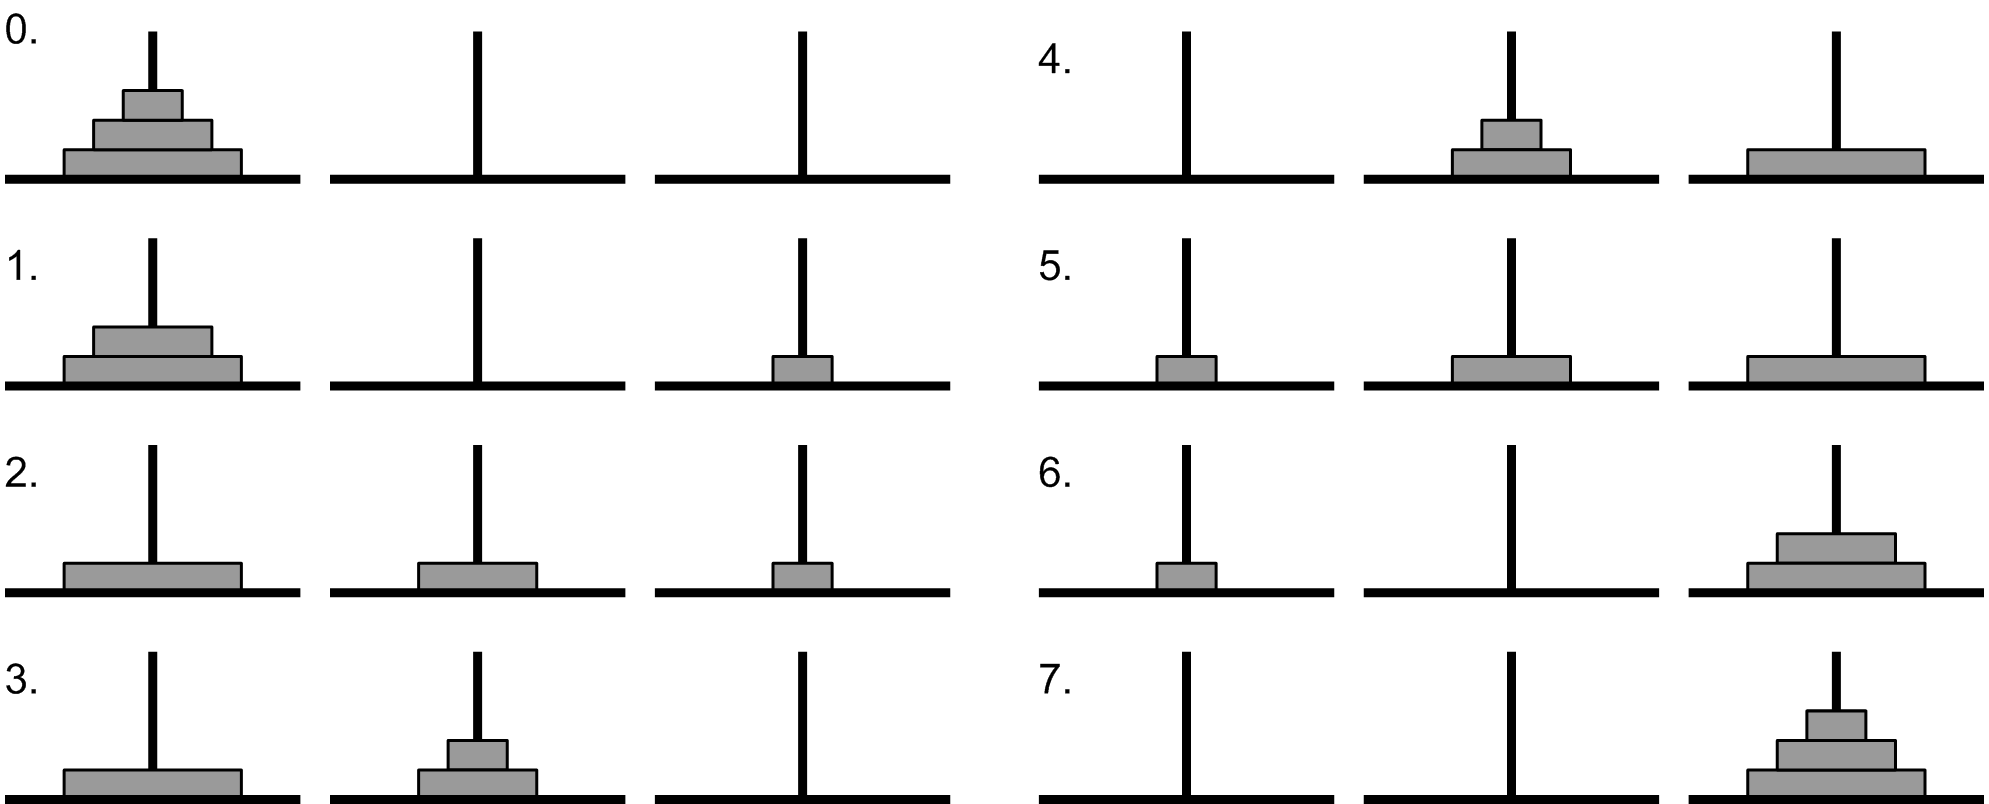
\includegraphics[scale=0.7]{hanoi.png}
	\end{center}
	\caption*{Solution to the Towers of Hanoi with 3 disks.}
	\label{fig:hanoi_solved}
\end{figure}

Solve the {\em Tower of Hanoi} puzzle for an arbitrary number of disks, enumerating the required moves.
